%%% lorem.tex --- 
%% 
%% Filename: lorem.tex
%% Description: 
%% Author: Ola Leifler
%% Maintainer: 
%% Created: Wed Nov 10 09:59:23 2010 (CET)
%% Version: $Id$
%% Version: 
%% Last-Updated: Tue Oct  4 11:58:17 2016 (+0200)
%%           By: Ola Leifler
%%     Update #: 7
%% URL: 
%% Keywords: 
%% Compatibility: 
%% 
%%%%%%%%%%%%%%%%%%%%%%%%%%%%%%%%%%%%%%%%%%%%%%%%%%%%%%%%%%%%%%%%%%%%%%
%% 
%%% Commentary: 
%% 
%% 
%% 
%%%%%%%%%%%%%%%%%%%%%%%%%%%%%%%%%%%%%%%%%%%%%%%%%%%%%%%%%%%%%%%%%%%%%%
%% 
%%% Change log:
%% 
%% 
%% RCS $Log$
%%%%%%%%%%%%%%%%%%%%%%%%%%%%%%%%%%%%%%%%%%%%%%%%%%%%%%%%%%%%%%%%%%%%%%
%%
%%% Code:


\chapter{Theory} \label{ch:theory}
Since several mesh simplification algorithms are being considered, \cref{sec:related_work} gives a brief overview of the most notable schemes found in previous work. A more detailed explanation of the algorithms can be found in \cref{sec:appearance-preserving_simplification,sec:quadric-based_error_metric,sec:progressive_meshes}.

Afterwards, in \cref{sec:metrics_for_appearance_preservation}, the different metrics that can be used to measure the appearance preservation after a simplification has been done is discussed. This will later be used to evaluate the solution empirically by giving a concrete metric for the amount of appearance deviation.

Finally, in \cref{sec:measuring_algorithmic_performance}, the methods and common practices for measuring performance of an algorithm are discussed. Based on existing industry practices, we show how to measure the computation time and memory usage of the algorithms. Since these measurements can be noisy, statistical methods will need to be used to truthfully answer our research questions.

%%%%%%%%%%%%%%%%%%%%%%%%%%%%%%%%%%%%%%%%%%%%%%%%%%%%%%%%%%%%%%%%%%%%%%
%%
%%% Related Work
%%
%%%%%%%%%%%%%%%%%%%%%%%%%%%%%%%%%%%%%%%%%%%%%%%%%%%%%%%%%%%%%%%%%%%%%%
\section{Related Work} \label{sec:related_work}
Some different approaches have been presented in the literature to solve the problem of simplifying a mesh. Early solutions focused on the geometrical error which is enough in many cases, but in the case of a mesh with appearance attributes this may give a poor result. Other solutions have been presented that takes the attributes into account to give a better appearance of the mesh. This section will give a brief overview of the simplification algorithms that can be found in the literature.

According to \emph{David Luebke's survey}~\cite{luebke2001developer} on the subject, mesh simplification is a technique which transforms a geometrically complex mesh (with a lot of polygons) to a simpler representation by removing unimportant geometrical details (reducing the number of polygons). It does this by assuming that some meshes are small, distant, or have areas which are unimportant to the visual quality of the rendered image. For example, if the camera in a scene always faces toward a certain direction, then removing details from the backside of a mesh won't affect the final rendered result, since they will never be seen by the camera anyway. Reducing the number of polygons allows meshes to use less storage space and need less computation time.

There are many mesh simplification algorithms, as can be seen in \emph{David Luebke's survey}~\cite{luebke2001developer}, each presenting a new approach with their own strengths and weaknesses. The first scheme is due to \emph{Schroeder et al.}~\cite{schroeder1992decimation} in 1992, called \emph{mesh decimation}. It was meant to be used to simplify meshes produced by the marching cubes algorithm, which usually gives unnecessary details. It works by making multiple passes through the meshes' vertices, and deleting vertices that do not destroy local topology and are within a given distance threshold when re-triangulated.

Besides \emph{decimation-based methods}, such as the aforementioned mesh decimation scheme, there exists another class of simplifiers based on \emph{vertex-merging mechanisms}. According to \emph{Luebke}~\cite{luebke2001developer}, these work by iteratively collapsing a pair of vertices \((v_j, v_k)\) into a single vertex \(v_i\). This will also remove any polygons which were suspended by \((v_j, v_k)\). The first collapse scheme is due to \emph{Hoppe et al.}~\cite{hoppe1993mesh}, which shows an \emph{edge collapse} of \(e_{ji} = (v_j, v_i) \rightarrow v_i\) as in \cref{fig:mesh_transformations} (a). There exist other schemes, such as \emph{pair contraction} in \cref{fig:mesh_transformations} (c) where vertices within a distance $t$ are allowed to be merged. These don't tend to preserve the local topology of the original mesh, and instead focus on a more aggressive simplification.

\begin{figure}[h]
    \centering
    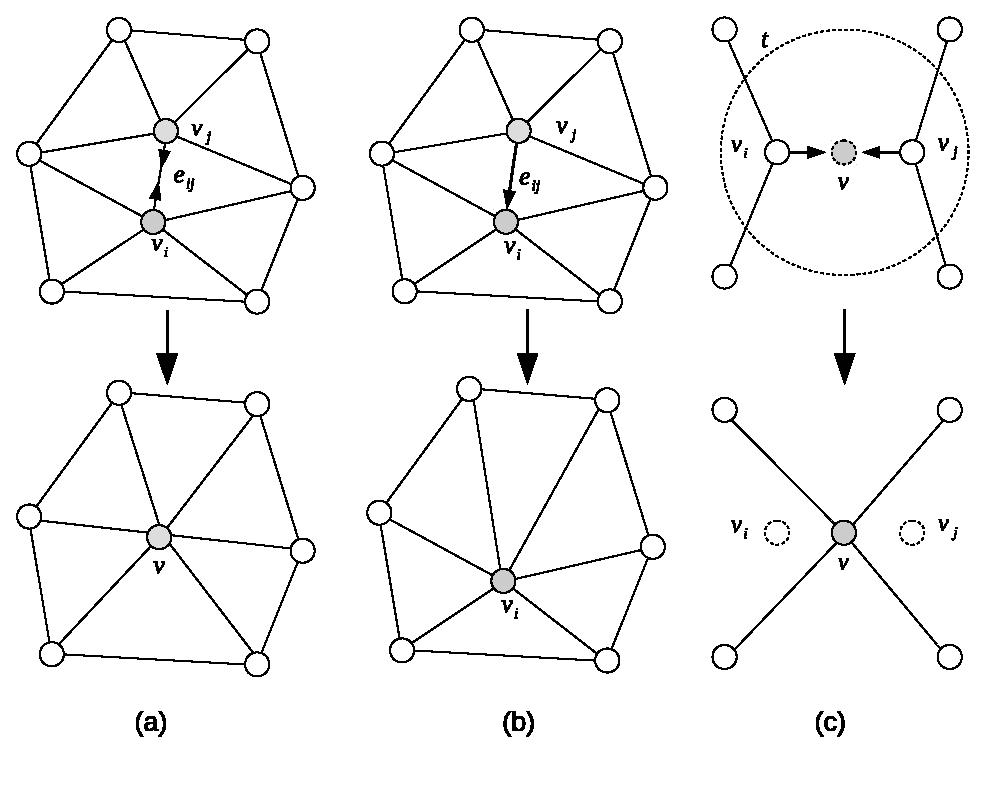
\includegraphics[width=\textwidth]{figures/mesh_transformations.eps}
    \caption{(a) edge collapse, (b) vertex removal, and (c) pair contraction}
    \label{fig:mesh_transformations}
\end{figure}

\emph{Quadric Error Metrics} (QEM), due to \emph{Garland and Heckbert} \cite{garland1997surface} performs edge collapses to provide a provably optimal simplification. In each iteration, an edge is collapsed \((v_j, v_i) \rightarrow \mathbf{v}\) and \(\mathbf{v}\) is repositioned at the position which gives the lowest possible geometrical error. \emph{Hoppe} \cite{hoppe1996progressive} also perform edge collapses but he tries to minimize an energy function. The edge with the lowest estimated energy is chosen for the collapse. 


%\subsection{Preserving appearance}
Focusing on minimizing the geometrical error during simplification works well for many meshes. But in the case of a mesh with appearance attributes such as color, normals, and texture coordinates the result may be poor. A common way to solve this is to use a metric which does not only take the geometry, but also the appearance attributes into account.

\emph{Cohen et al.} \cite{cohen1998appearance} defines a new \emph{texture deviation metric} which takes three attributes into account: Surface position, surface curvature, and surface color. These attributes are sampled from the input surface and the simplification is done with edge collapses and vertex removals.

\emph{Sander et al.} \cite{sander2001texture} uses the texture deviation metric together with a \emph{texture stretch metric} to better balance frequency content in every direction all over the surface.

An extended more general version of the QEM is presented by \emph{Garland and Heckbert} \cite{garland1998simplifying} where the metric can be used for points in $n$-dimensional space. Thus, when the color is considered each vertex would be represented by a 6-dimensional vector. Another version of QEM by \emph{Hoppe} \cite{Hoppe:1999:NQM:319351.319357} base the attribute error on geometric correspondence in 3D rather than using points in $n$-dimensional space.

\emph{Image-driven simplification} defined by \emph{Lindstrom and Turk} \cite{lindstrom2000image} captures images from different angles of the mesh. The distance between images of the mesh before and after an edge collapse are used to guide the simplification.

\iffalse %%%%%%%%%%%%%%%%%%%%%

============================
 Mesh simplification
============================
* Geometry
  - Mesh decimation
  - Mesh optimization
  - Progressive meshes
  - Surface simplification using quadric error metric
  
* Geometry and appearance attributes
  - Appearance-preserving simplification

  - Texture mapped progressive meshes
  
  - Simplifying surfaces with color and texture using quadric error metric
  - New quadric error metric

  - Image-driven simplification

============================
 Mesh parametrization
============================
  Resample texture
  Ray tracing
  Volume UV
  
\fi %%%%%%%%%%%%%%%%%%%%%%%%%%
  
\iffalse %%%%%%%%%%%%%%%%%%%%%
\section{Mesh Transformations} \label{sec:mesh_transformations}
The detail of a mesh can be reduced/increased by altering the vertices and edges of the mesh. There exist several mechanisms that can be used.

\begin{itemize}
\item Edge collapsing
\item Vertex removal
\item Pair contraction
\item Vertex split
\end{itemize}

In edge collapsing, the vertices of the edge $e_{ij} = (v_i, v_j)$ is removed and replaced with a single vertex $v$ somewhere in between. The triangles that used the edge $e_{ij}$ is removed and the neighbors of $v_i, v_j$ will be connected with the new created vertex. This can be seen in \cref{fig:mesh_transformations}(a).

Vertex removal is similar to edge collapsing, but now only one vertex is removed and the other vertex is moved to the location of the removed vertex. The neighbors of the removed vertex will be connected to the one that remains. In ~\cref{fig:mesh_transformations}(b) vertex $v_j$ of edge $e_{ji}$ is removed and vertex $v_i$ is moved to the location of $v_j$.

In a pair contraction, it is possible to merge two distant vertices that are not connected by an edge. Usually, the vertices have to within a certain threshold to be considered for a contraction. In \cref{fig:mesh_transformations}(c) the vertices $v_j, v_k$ is contracted into the new vertex $v_i$. 

To increase the detail of the mesh an existing vertex can be split into two, i.e. vertex split. When performing a vertex split a vertex $v$ is split into two new vertices $v_i, v_j$ connected by an edge $e_{ij}$. 

\begin{figure}[h]
    \centering
    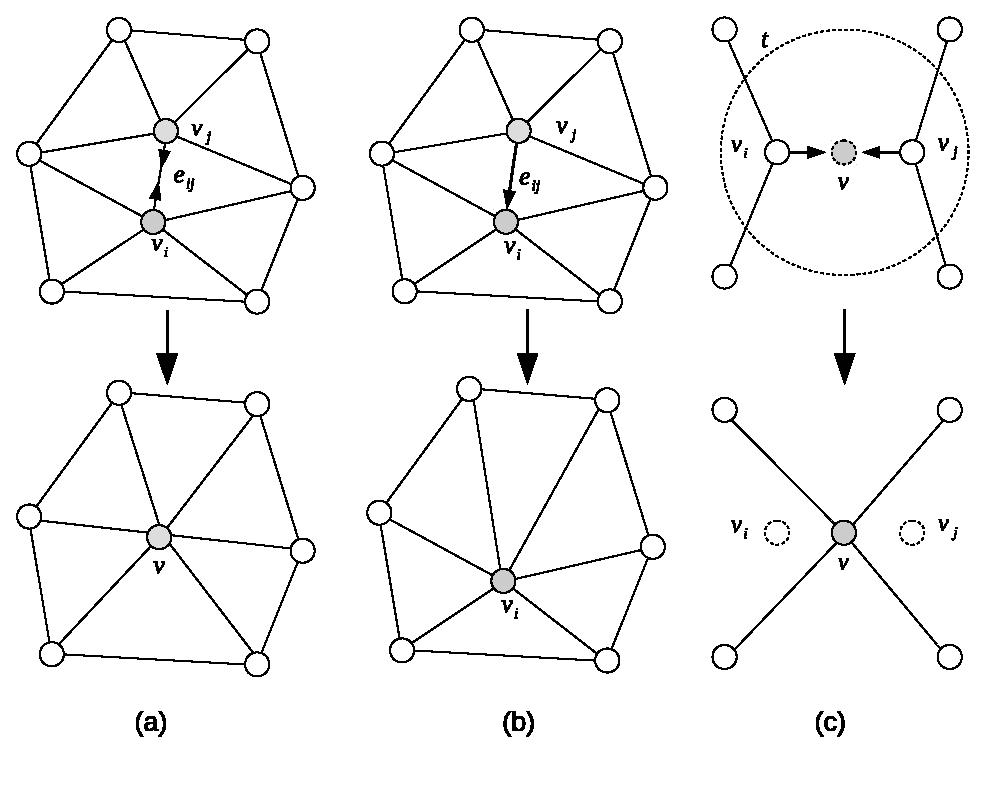
\includegraphics[width=\textwidth]{figures/mesh_transformations.eps}
    \caption{(a) edge collapse, (b) vertex removal, and (c) pair contraction}
    \label{fig:mesh_transformations}
\end{figure}
\fi %%%%%%%%%%%%%%%%%%%%%%%%%%

%%%%%%%%%%%%%%%%%%%%%%%%%%%%%%%%%%%%%%%%%%%%%%%%%%%%%%%%%%%%%%%%%%%%%%
%%
%%% Appearance-Preserving simplification
%%
%%%%%%%%%%%%%%%%%%%%%%%%%%%%%%%%%%%%%%%%%%%%%%%%%%%%%%%%%%%%%%%%%%%%%%
\section{Appearance-Preserving Simplification} \label{sec:appearance-preserving_simplification}
In order to preserve the appearance of a model when it is simplified, \emph{Cohen et al.} \cite{cohen1998appearance} defines a \emph{texture deviation metric}. This metric takes three attributes into account: Surface position, surface curvature, and surface color. To properly sample these attributes from the input surface, the surface position is decoupled from the color and normals stored in texture and normal maps, respectively. The metric guarantees that the maps will not shift more than a user-specified number of pixels on the screen. This user-specified number is defined as $\epsilon$.

Approximation of the surface position is done offline with simplification operations such as edge collapsing and vertex removals. At run-time, the color and normals are sampled in pixel-coordinates with mip-mapping techniques. Mip-maps are a pre-calculated sequence of images with progressively lower resolution. Here the decoupled representation is useful since the texture deviation metric can be used to bound how much the mapped attributes value's positions deviate from the positions of the original mesh. This guarantees that the sampling and mapping to screen-space of the attributes is done in an appropriate way.

Before any simplification can be made, a parametrization of the surface is required in order to store the color and normals in maps. If the input mesh does not have a parametrization, it is created and stored per-vertex in texture and normal maps. Next, the surface and maps are fed into the simplification algorithm which decides which simplification operations to use and in what order. The deviation caused by each operation is measured with the texture deviation metric. A \emph{progressive mesh} (PM) with error bounds for each operation is returned by the algorithm, which can then be used to create a set of LOD with error bounds. Using the error bounds, the tessellation of the model can be adjusted to meet the user-specified error $\epsilon$.

%%%%%%%%%%%%%%%%%%%%%%%%%%%%%%%%%%%%%%%%%%%%%%%%%%%%%%%%%%%%%%%%%%%%%%
%%
%%% Quadric-Based Error Metric
%%
%%%%%%%%%%%%%%%%%%%%%%%%%%%%%%%%%%%%%%%%%%%%%%%%%%%%%%%%%%%%%%%%%%%%%%
\section{Quadric-Based Error Metric} \label{sec:quadric-based_error_metric}
% Surface simplification using quadric error metric
\iffalse %%%%%%%%
\begin{figure}[ht]
    \centering
    \begin{minipage}{0.49\textwidth}
        \centering
        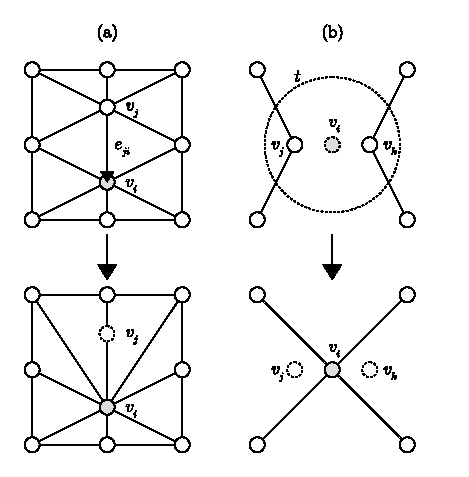
\includegraphics[width=\textwidth]{figures/contraction_types.eps}
        \caption{(a) edge \(e_{ji} = (v_j, v_i)\) contraction toward \(v_i\)
                 and (b) pair \((v_j, v_k)\) contraction in the distance threshold \(t\) toward new vertex \(v_i\).}
        \label{fig:contractions}
    \end{minipage} \hfill
    \begin{minipage}{0.485\textwidth}
        \centering
        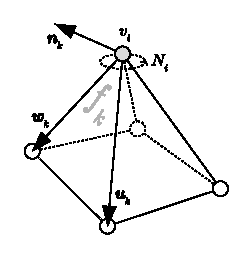
\includegraphics[width=\textwidth]{figures/quadric_planes.eps}
        \caption{Depiction of one of the planes \(f_k\) in the neighborhood \(N_i\) of the vertex \(v_i\). It has a normal \(\mathbf{n}_k\); found by the \(\mathbf{w}_k \times \mathbf{u}_k\) of its edges.}
        \label{fig:quadrics}
    \end{minipage}
\end{figure}
\fi %%%%%%%%%

Mesh simplification with \emph{Quadric Error Metrics} (QEM), due to \emph{Garland and Heckbert}~\cite{garland1997surface}, is based on the vertex merging paradigm. It provides a provably optimal simplification in each iteration, by collapsing the edge \((v_j, v_i) \rightarrow v_i\) and re-positioning it at \(\mathbf{v}\), which gives it the lowest possible geometrical error. By assigning a matrix \(\mathbf{Q}_i\) for each vertex \(v_i\), one can find the error \(\mathup\Delta(\mathbf{v})\) introduced by moving \(v_i\) to \(\mathbf{v}\). \(\mathup\Delta(\mathbf{v})\) is the sum of squared distances from \(\mathbf{v}\) to the planes \(\mathbf{f}_k\) in \(v_i\)'s neighborhood \(N_i\) (all polygons around \(v_i\) as in \cref{fig:quadrics}).

\begin{figure}[ht]
  \centering
  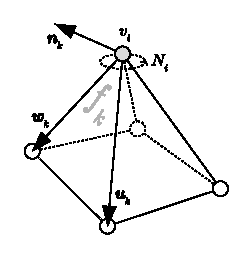
\includegraphics[width=0.4\textwidth]{figures/quadric_planes.eps}
  \caption{Depiction of one of the planes \(f_k\) in the neighborhood \(N_i\) of the vertex \(v_i\). It has a normal \(\mathbf{n}_k\); found by the \(\mathbf{w}_k \times \mathbf{u}_k\) of its edges.}
  \label{fig:quadrics}
\end{figure}

%\vspace{-0.7em}

Since \(\mathup\Delta(\mathbf{v})\) is quadratic, finding a \(\mathbf{v}\) which gives a minimal error is a linear problem. The best position \(\mathbf{\overline{v}}_i\) for \(v_i\) after a collapse \((v_j, v_i) \rightarrow v_i\) is a solution to \cref{eq:quadric_opt}.

\begin{equation} \label{eq:quadric_opt}
(\mathbf{Q}_j + \mathbf{Q}_i)\mathbf{\overline{v}}_i = \begin{bmatrix} 0 & 0 & 0 & 1 \end{bmatrix}\transpose.
\end{equation}

\begin{equation} \label{eq:homogeneous_quadric}
      \mathup\Delta(\mathbf{v}) = \mathbf{v}\transpose \mathbf{Q}_i  \mathbf{v} \;,\;\; \mathbf{Q}_i = \sum_{f_k \in N_i}  \mathbf{f_k} \mathbf{f_k}\transpose \; .
\end{equation}

By storing the \(\mathup\Delta(\mathbf{\overline{v}}_i)\) for every valid collapse \((v_j, v_i) \rightarrow v_i\) in a min-heap, the least cost collapse on the top of the heap can be done in each iteration, removing a vertex in each step. This is repeated until either a user-given vertex count \(|\mathcal{V}|\) is reached or until some error threshold \(\epsilon\).

The results by \emph{Garland and Heckbert}~\cite{garland1997surface} show that QEM can reduce the simplification error by up to 50 \% in comparison to a na\"ive scheme where \(\mathbf{\overline{v}}_i = (v_i + v_j) / 2\) and \(\Delta(\mathbf{\overline{v}}_i) = ||\mathbf{\overline{v}}_i - v_i||\). They also argue that QEM gives higher-quality simplifications than \emph{vertex clustering} and that it is faster than \emph{progressive meshing} (which we also present later).

\iffalse
\begin{figure}[ht]
    \centering
    \includegraphics[width=\textwidth]{figures/naive_simplification.png}
    \includegraphics[width=\textwidth]{figures/quadric_simplification.png}
    \caption{Simplification using a na\"ive (top image) and a quadric error metric (bottom image) at different levels of detail at some vertex count (left to right: 50 \%, 35 \% and 17 \% of original).}
    \label{fig:naive_vs_quadric}
\end{figure}
\fi

%Simplifying surfaces with color and texture using quadric error metrics
%\subsection{Preserving appearance}
A general version of QEM was later presented by Garland and Heckbert \cite{garland1998simplifying} where vertices can be placed in $n$-dimensional space. This makes it possible to, for example, include the color of the surface in the computation. Each vertex is treated as a vector \(v \subset \mathbb{R}^n\). Thus, when the color is considered each vertex will be represented by a 6-dimensional vector \(v = [x, y, z, r, g, b]\transpose\). The first three values is the spatial coordinates and the last three values will be the color. The same thing can be done with for example texture coordinates where each vertex would be represented by a 5-dimensional vector \(v = [x, y, z, s, t]\transpose\) where $s, t$ is the 2D texture coordinates.

The original version of QEM used a 4x4 homogeneous matrix $Q_i$ for the computations. A more convenient notation is used in the general version. A face in the original model defines a plane which satisfies the equation \(\mathbf{n}\transpose \mathbf{v} + d = 0\) where \(\mathbf{n}\) is the face normal and \(d\) is a scalar. The squared distance of a vertex to a plane is given by
\begin{equation}
  D^2 = (\mathbf{n}\transpose\mathbf{v} + d)^2 = \mathbf{v}\transpose(\mathbf{nn}\transpose)\mathbf{v} + 2d\mathbf{n}\transpose\mathbf{v} + d^2
\end{equation}

$D^2$ can now be represented as the quadric Q
\begin{equation}
  Q = (\mathbf{A}, \mathbf{b}, c) = (\mathbf{nn}\transpose, d\mathbf{n}, d^2)
\end{equation}
\begin{equation}
  Q(\mathbf{v}) = \mathbf{v}\transpose\mathbf{Av} + 2\mathbf{bv} + c
\end{equation}


where \(Q(\mathbf{v})\) is the sum of squared distances. This representation performs matrix operations on 3x3 matrices instead of 4x4 as in the previous notation. This increases performance when, for example, performing matrix inversions.

The overhead of the higher dimensional quadrics is not extreme according to Garland and Heckbert. However, when using this with colors, normals, and texture coordinates some caution is needed. Colors may need to be clamped and normals needs to be normalized to unit length.

Garland and Heckbert have assumed that the properties vary continuously over the whole surface. However, if we want to for example apply a texture to a cylinder there will always be a seam where the ends of the texture meets. All vertices along this seam needs to be duplicated since they would require two different texture coordinates. The authors suggested having boundary constraints that would maintain the seam. However, in the case where a mesh have a corresponding texture atlas where each face have a specific part of the texture this might not work. The solution suggested by the authors is to allow multiple quadrics for each vertex, but, this is not yet implemented.

%New quadric error metric
Hugues Hoppe \cite{Hoppe:1999:NQM:319351.319357} also uses QEM for meshes with appearance attributes. Instead of calculating the distances to hyperplanes as Garland and Heckbert, Hoppe base the attribute error on geometric correspondence in 3D. A point \(\mathbf{p}\) is projected onto a face in \(\mathbb{R}^3\) rather than a plane in a higher dimension and then both the geometric and attribute error is computed. According to the author this gives a better result compared to Garland and Heckberts general QEM.

%%%%%%%%%%%%%%%%%%%%%%%%%%%%%%%%%%%%%%%%%%%%%%%%%%%%%%%%%%%%%%%%%%%%%%
%%
%%% Progressive Meshes
%%
%%%%%%%%%%%%%%%%%%%%%%%%%%%%%%%%%%%%%%%%%%%%%%%%%%%%%%%%%%%%%%%%%%%%%%
\section{Progressive Meshes} \label{sec:progressive_meshes}
Hugues Hoppe \cite{hoppe1996progressive} introduced the \emph{Progressive Mesh} (PM) representation as a scheme for storing and transmitting arbitrary polygon meshes. An arbitrary mesh $\hat{M}$ in PM form is defined by a sequence of meshes $M^0, M^1, ..., M^n$ with increasing accuracy of the original mesh $\hat{M} = M^n$. Only the most coarse mesh $M^0$ is stored together with records of \emph{vertex splits} that is used to refine $M^0$ into the more detailed meshes. A vertex split will transform $M^i$ the more detailed mesh $M^{i+1}$ and an edge collapse transforms $M^i$ to the coarser mesh $M^{i-1}$.

To construct a PM the edge collapses of the original mesh needs to be determined. Multiple possible algorithms for choosing those edge collapses is presented by Hoppe \cite{hoppe1996progressive}, some with high speed but low accuracy and some more accurate but with lower speed. A fast but maybe not so accurate strategy is to choose the edge collapses at random but with some conditions. Another more accurate scheme is to use heuristics. According to Hoppe, the construction of a PM is supposed to be a preprocess, Therefore, the author chose an algorithm that take some time but is more accurate.

Hoppe based the simplification on the previous work \emph{Mesh Optimization} \cite{hoppe1993mesh} where the goal is to find a mesh that fits a sets $X$ of points \(x_i \subset \mathbb{R}^3\) with a small number of vertices. This problem is defined as a minimization of the energy function.
\begin{equation}
  E(M) = E_{dist}(M) + E_{spring}(M) + E_{scalar}(M) + E_{disc}(M)n
\end{equation}

\emph{Distance energy} $E_{dist}(M)$ measures the sum of the squared distances from the points to the mesh. \emph{Spring energy} $E_{spring}$ is used to regularize the optimization problem. \emph{Scalar energy} $E_{scalar}$ measures the accuracy of the scalar attributes of the mesh. The last term, $E_{disc}$ measures the geometric accuracy of the discontinuity curves (e.g creases). All legal edge collapses is placed in a priority queue where the edge collapse with lowest $\mathup\Delta E$ (estimated energy) is on the top of the queue. After a transformation is performed, the energy of the neighboring edges is updated.

%\subsection{Preserving appearance} \label{sec:texture_mapped_progressive_meshing}
Given an arbitrary mesh, \emph{Sander et. al} \cite{sander2001texture} presents a method to construct a PM where a texture parametrization is shared between all meshes in the PM sequence. In order to create a texture mapping for a simplified mesh, the original mesh's attributes, e.g normals, is sampled. This method was developed with two goals taken into consideration:
\begin{itemize}
\item{Minimize \emph{texture stretch}:}~~~When a mesh is simplified the texture may be stretched in some areas which decrease the quality of the appearance. Since the texture parametrization determines the sampling density, a balanced parametrization is preferred over one that samples with different density in different areas. The balanced parametrization is obtained by minimizing the largest texture stretch over all points in the domain. No point in the domain will therefore be too stretched and thus making no point undersampled. 
\item{Minimize \emph{texture deviation}:}~~~Conventional methods use geometric error for the mesh simplification. According to the authors this is not appropriate when a mesh is textured. The stricter texture deviation error metric, where the geometric error is measured according to the parametrization, is more appropriate. This is the metric by \emph{Cohen et al.} \cite{cohen1998appearance} explained in \cref{sec:appearance-preserving_simplification}. By plotting a graph of the texture deviation vs the number of faces, the goal is to minimize the height of this graph.
\end{itemize}

\emph{Cohen et al.} \cite{cohen1998appearance} stored an error bound for each vertex in a PM. \emph{Sander et al.} \cite{sander2001texture} instead tries to find an atlas parametrization that minimizes both texture deviation and texture stretch for all meshes in the PM.

%%%%%%%%%%%%%%%%%%%%%%%%%%%%%%%%%%%%%%%%%%%%%%%%%%%%%%%%%%%%%%%%%%%%%%
%%
%%% Mesh parameterization
%%
%%%%%%%%%%%%%%%%%%%%%%%%%%%%%%%%%%%%%%%%%%%%%%%%%%%%%%%%%%%%%%%%%%%%%%
\section{Mesh Parameterization} \label{sec:mesh_parametrization}
In order to apply, for example, a texture to a mesh each vertex is given a texture coordinate. This problem of finding a mapping between a surface (mesh)and a parameter domain (texture map) is called parameterization. Given a triangular mesh Hormann et al. \cite{hormann2007mesh} refers to the mapping problem as mesh parameterization. According to Hormann et al. there exists a one-to-one mapping between two surfaces with similar topology. Thus, a surface that is homeomorphic to a disk can be mapped onto a plane, i.e. a texture. If a mesh is not homeomorphic to a disk it has to be split into parts which are homeomorphic to a disk. These parts can then be put onto the same plane and only one texture is needed.

%%%%%%%%%%%%%%%%%%%%%%%%%%%%%%%%%%%%%%%%%%%%%%%%%%%%%%%%%%%%%%%%%%%%%%
%%
%%% Multiple attributes for a vertex
%%
%%%%%%%%%%%%%%%%%%%%%%%%%%%%%%%%%%%%%%%%%%%%%%%%%%%%%%%%%%%%%%%%%%%%%%
\section{Multiple attributes for a vertex} \label{sec:vertex_with_multi_attributes}
A vertex of a mesh often have a properties associated with it such as texture coordinates, color, and normal. A common way of texturing a model is to use a texture atlas where each triangle of the mesh is assigned a specific part of the texture. Since a texture is in a 2-dimensional domain a mesh parameterization needs to be performed. In many cases the mesh needs to be cut somewhere which will create seams. The vertices along this seam would require two sets of texture coordinates and this will create a discontinuity. In \cref{fig:cylinder_unwrap} a cylinder is unwrapped to 2D which creates a seam. All vertices along the seam will have two sets of texture coordinates $(s,t)$, one with $s=0$ and a second with $s=1$.


\begin{figure}[ht]
    \centering
    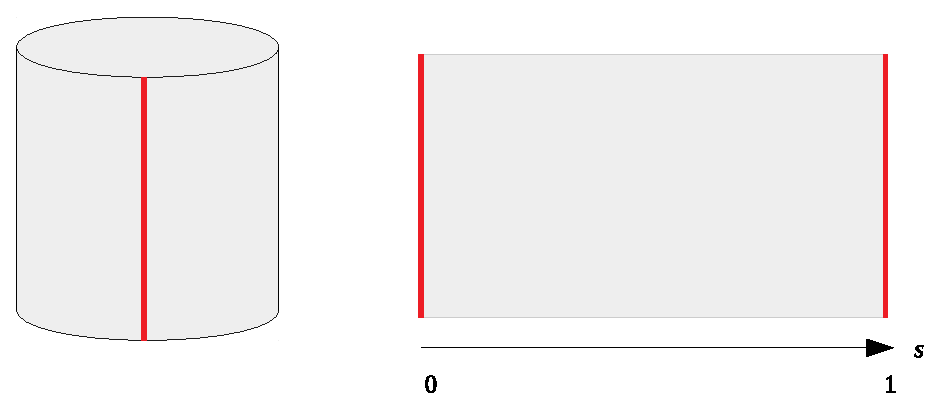
\includegraphics[width=.8\textwidth]{figures/cylinder_unwrap.eps}
    \caption{Unwrapping a cylinder. Vertices along seam (red line) require two texture coordinates}
    \label{fig:cylinder_unwrap}
\end{figure}


Hugues Hoppe \cite{hoppe1998efficient} presents a mesh representation where each face adjacent to a vertex can have different appearance attributes. The attribute values is associated with the corners of the faces instead of the vertices. A \emph{corner} is defined by Hoppe as a tuple $<vertex,face>$. The attribute values at a corner defines the value that should be used for face $f$ at vertex $v$. Corners with the same attributes and adjacent vertex are stored in a \emph{wedge}. The wedge has one or more corners and each vertex will be divided into one or more wedges. This representation is useful for simplification of meshes with discontinuities in their attribute fields. Discontinuities could result in a simplified mesh where adjacent faces have been separated which introduces new holes in the mesh.

\begin{figure}[ht]
    \centering
    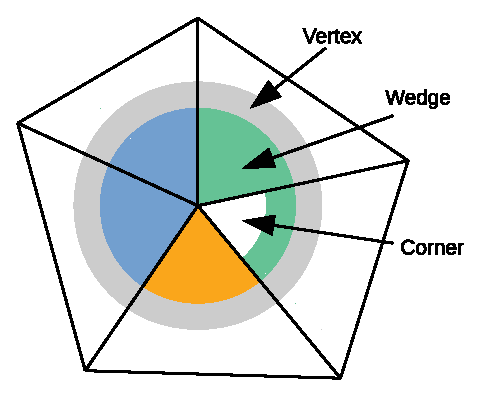
\includegraphics[width=.49\textwidth]{figures/wedge.eps}
    \caption{Vertex with wedges}
    \label{fig:wedge}
\end{figure}

%%%%%%%%%%%%%%%%%%%%%%%%%%%%%%%%%%%%%%%%%%%%%%%%%%%%%%%%%%%%%%%%%%%%%%
%%
%%% Metric for Appearance Preservation
%%
%%%%%%%%%%%%%%%%%%%%%%%%%%%%%%%%%%%%%%%%%%%%%%%%%%%%%%%%%%%%%%%%%%%%%%
\section{Metrics for Appearance Preservation} \label{sec:metrics_for_appearance_preservation}
Previously in \cref{sec:appearance-preserving_simplification,sec:progressive_meshes}, the metrics texture deviation and texture stretch have been defined. But to measure more exactly how much the visual appearance of a simplified mesh deviate from the original mesh another metric would be better. \emph{Lindstrom and Turk} \cite{lindstrom2000image} defines \emph{image-driven simplification} which captures images from different angles of the mesh. The difference between the images of the original and simplified mesh are computed in order to measure how well the appearance is preserved. This metric is more general and can be applied to all simplification algorithms since it only compares the original mesh to the simplified mesh.

The \emph{image metric} is defined as a function taking two images and gives the distance between them. To measure the distance the authors use root mean square of the luminance values of two images $Y^0$ and $Y^1$ with dimensions $m \times n$ pixels. It is defined as:
\begin{equation} \label{eq:rms_images}
  d_{RMS}(Y^0,Y^1) = \sqrt{\tfrac{1}{mn}\sum^m_{i=1}\sum^n_{j=1}(y^0_{ij} - y^1_{ij})^2}
\end{equation}

To evaluate the quality of the simplified mesh the authors capture images from 24 different camera positions. The positions are defined as the vertices of a rhombicuboctahedron which can be seen in \cref{fig:rhombicuboctahedron}. Two sets of $l$ images $Y^0 = {Y^0_h}$ and $Y^1 = {Y^1_h}$ with dimensions $m \times n$ is rendered and the RMS is then computed as:
\begin{equation}  \label{eq:rms_image_sets}
  d_{RMS}(Y^0,Y^1) = \sqrt{\tfrac{1}{lmn}\sum^l_{h=1}\sum^m_{i=1}\sum^n_{j=1}(y^0_{hij} - y^1_{hij})^2}
\end{equation}

\begin{figure}[h]
    \centering
    \includegraphics[width=0.25\textwidth]{figures/591px-Rhombicuboctahedron.jpg}
    \caption{Rhombicuboctahedron with 24 vertices which is used as the camera positions. 
      (\href{https://commons.wikimedia.org/wiki/File:Rhombicuboctahedron.jpg}{Rhombicuboctahedron} by Hellisp / \href{https://creativecommons.org/licenses/by/3.0/}{CC BY 3.0})}
    \label{fig:rhombicuboctahedron}
\end{figure}

\section{Measuring Algorithmic Performance} \label{sec:measuring_algorithmic_performance}

According to \emph{David Lilja}~\cite[p.~4]{lilja2005measuring}, there are three fundamental techniques that can be used when confronted with a performance-analysis problem: \emph{measurement}, \emph{simulation} or \emph{modeling}. While the book concentrates on evaluating computer performance, these techniques can also be applied when evaluating different algorithms. Measurement would be to actually execute the implemented algorithm and simultaneously gather interesting statistics (e.g. how long it took to finish and how much memory was needed), and use this to compare the algorithms. While modeling would be to analytically derive an abstract model for the algorithm (e.g. the Big \(\mathcal{O}\) worst-case running time and memory), and see which of them has a lower complexity.

Since not all of the algorithms in \cref{sec:related_work} have an analytical model derived by the authors, and also because the algorithms are to be evaluated in a real system, only the problems inherent to the measurement approach will be considered. One of the problems with doing measurements of a real system (a program running on a computer in this case), according to \emph{David Lilja}~\cite[p.~43]{lilja2005measuring}, is that they introduce noise. This noise needs to be modeled to be able to reach a correct conclusion, such as determining if algorithm A is faster than algorithm B. One way of doing this, according to \emph{David Lilja}~\cite[p.~48]{lilja2005measuring}, is to find the confidence interval of the measured value, by assuming the source's error is distributed according to some statistical distribution (like the Gaussian or the Student t-distribution). The confidence interval \([a,b]\) when assuming the source's error is t-distributed, can be found as shown below. Where \(n\) tests are taken (giving \(n-1\) degrees of freedom), with a significance level of \(\alpha\) (usually 5 \%).

\begin{equation} a = \overline{x} - t_k\frac{s}{\sqrt{n}}, \quad
   b = \overline{x} + t_k\frac{s}{\sqrt{n}}, \quad
t_k = t_{1-\alpha/2,n-1} \end{equation}

One common mistake, according to \emph{Schenker et al.}~\cite{schenker2001judging}, when using confidence intervals to determine if e.g. an implemented algorithm A is faster than B, is the use of the overlapping method to reach conclusions. If two confidence intervals \emph{do not} overlap, then the result is provably significant (that is, algorithm A is either faster or slower than B). However, the converse is not true, if two intervals \emph{do} overlap, then no conclusions can be reached since the result could be either significant or not significant.

%%%%%%%%%%%%%%%%%%%%%%%%%%%%%%%%%%%%%%%%%%%%%%%%%%%%%%%%%%%%%%%%%%%%%%
%%% theory.tex ends here

%%% Local Variables: 
%%% mode: latex
%%% TeX-master: "thesis"
%%% End: 
